%===============================================================================
% Autoři: Michal Bidlo, Bohuslav Křena, Jaroslav Dytrych, Petr Veigend a Adam Herout 2018
\chapter{Úvod}
Aproximácie, ktoré ako inžinieri používame, nám často zjednodušujú prácu, no zároveň nám pília konár
pod nohami v prípadoch, keď vyžadujeme neomylnosť a presnosť.
Obdobná situácia sa vyskytuje aj v optike. Aberácie predstavujú odchýlky, ktoré vznikajú zjedošením
modelu optických systémov. Ich nesprávne pochope, či dokonca ignorácia, môže viesť k fatálnym chybám
ako napríklad v prípade Hubblového vesmírneho teleskopu.

\section{Aberácie}
Aberácie prestavujú odchýlky od bežného optického modelu, ktoré sú spôsobené zjednodušením
formalizov oproti realite. Príkladom je Schnellow zákon, ktorého bežná forma popisuje lom svetla len
pre tzv. paraxiálne uhly. \cite{hechtoptics}

Dôsledkom aberácii sú optické vady, ktoré sa prejavujú rozmazaním alebo deformáciou obrazu. V praxi sa tieto
vady riešia rozšírením optickej sústavy o ďalšie prvky, ktoré korigujú ľúče, prípadne pomocou
špecializovaných softwareov.

\section{Monochromatické aberácia}
Monochromatické aberácie predstavujú odchýlky, ktoré sa vyskytujú už pri jednej vlnovej dĺžke.
\subsection{Sférická aberacia}
Sférická aberácia nastáva pri dopade rovnobežných ľúčov na sférický rozhranie prostredí. 
Podľa bežnej teórie sa pri dopade na rozhranie zakrivenej šošovky láme ľúč do ohniska šošovky, ktoré
dané krivosťou danej šošovky. 
Pri dopade sa smer lomu riadi rozšírených Schnellovým zákonom, ktorý je rozšírený o odchýľkový člen, závislý na
uhle. Odchýlka uhlu pri lome spôsobuje, že ľúče nedopadajú do jedného ohniska šošovky, ale sú
rozptýlené v jeho okolí. Táto situácia
je zobrazená na obrázku \ref{saill}.

\begin{figure}[h]
\centering
\label{saill}
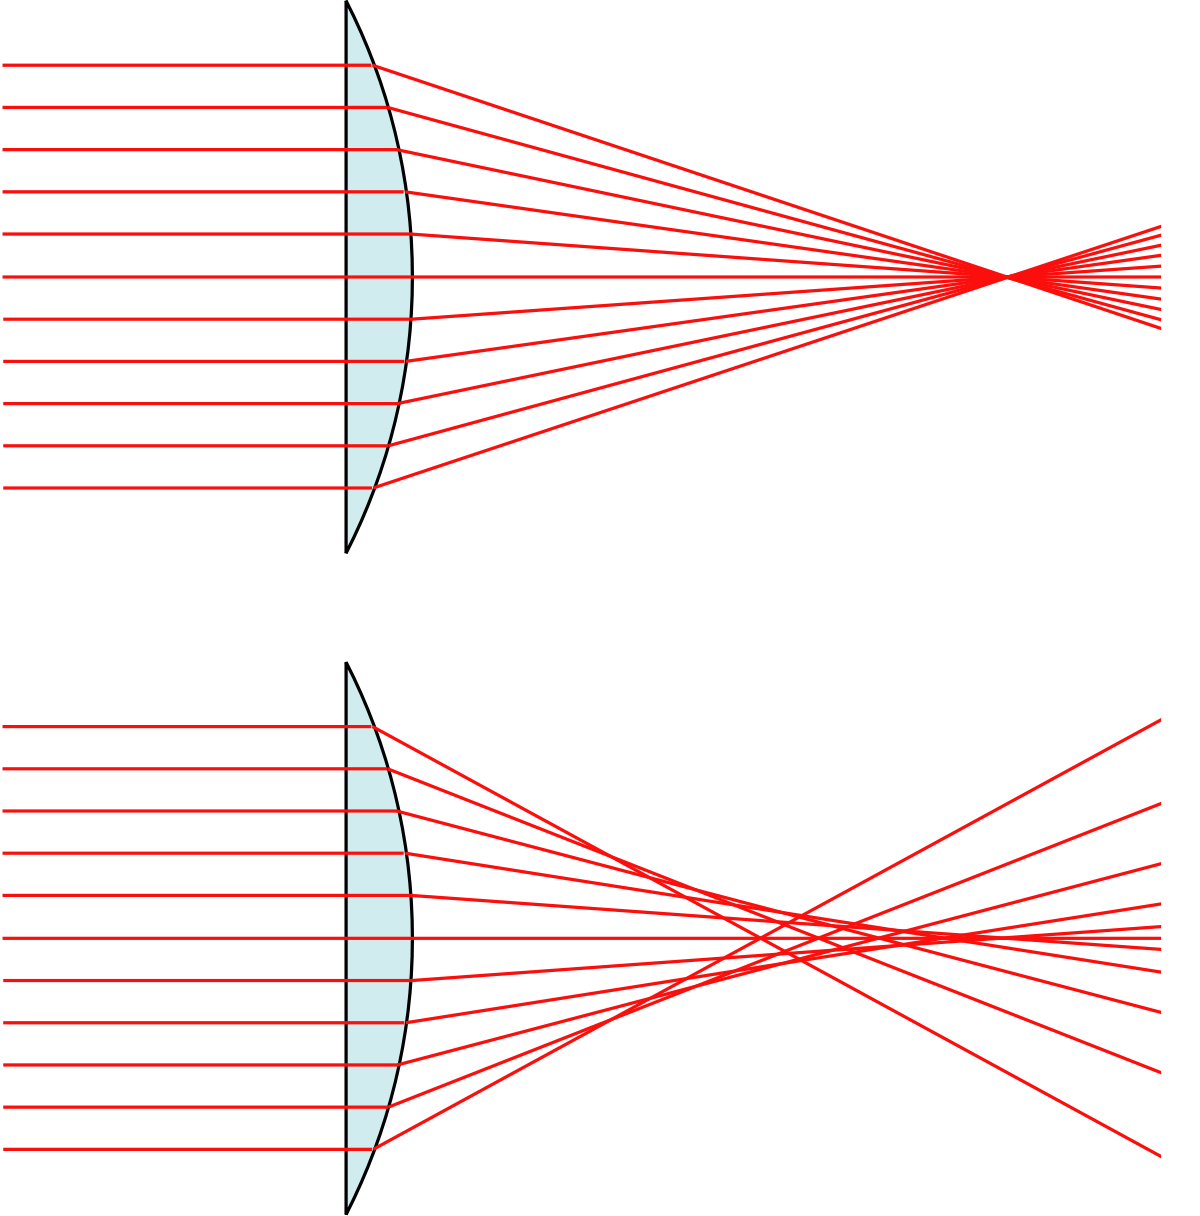
\includegraphics[width=6cm]{obrazky-figures/sphericalAberrationWikipedia.png}
\caption{Ilustrácia sférickej odchíľky. Vplyvom odchíľkového člena sa ľúče na rozhraní nelámu smerom
    do jedného ohniska. Prevzaté z }
\end{figure}

Dôsledkom tohoto javu je rozostretie obrazu pri okrajoch obrazu.  
Riešenie pomocou odlišného tvaru šošovky (apheric lens), ktoré sú ale drahé. https://en.wikipedia.org/wiki/Aspheric\_lens

\begin{figure}[h]
\centering
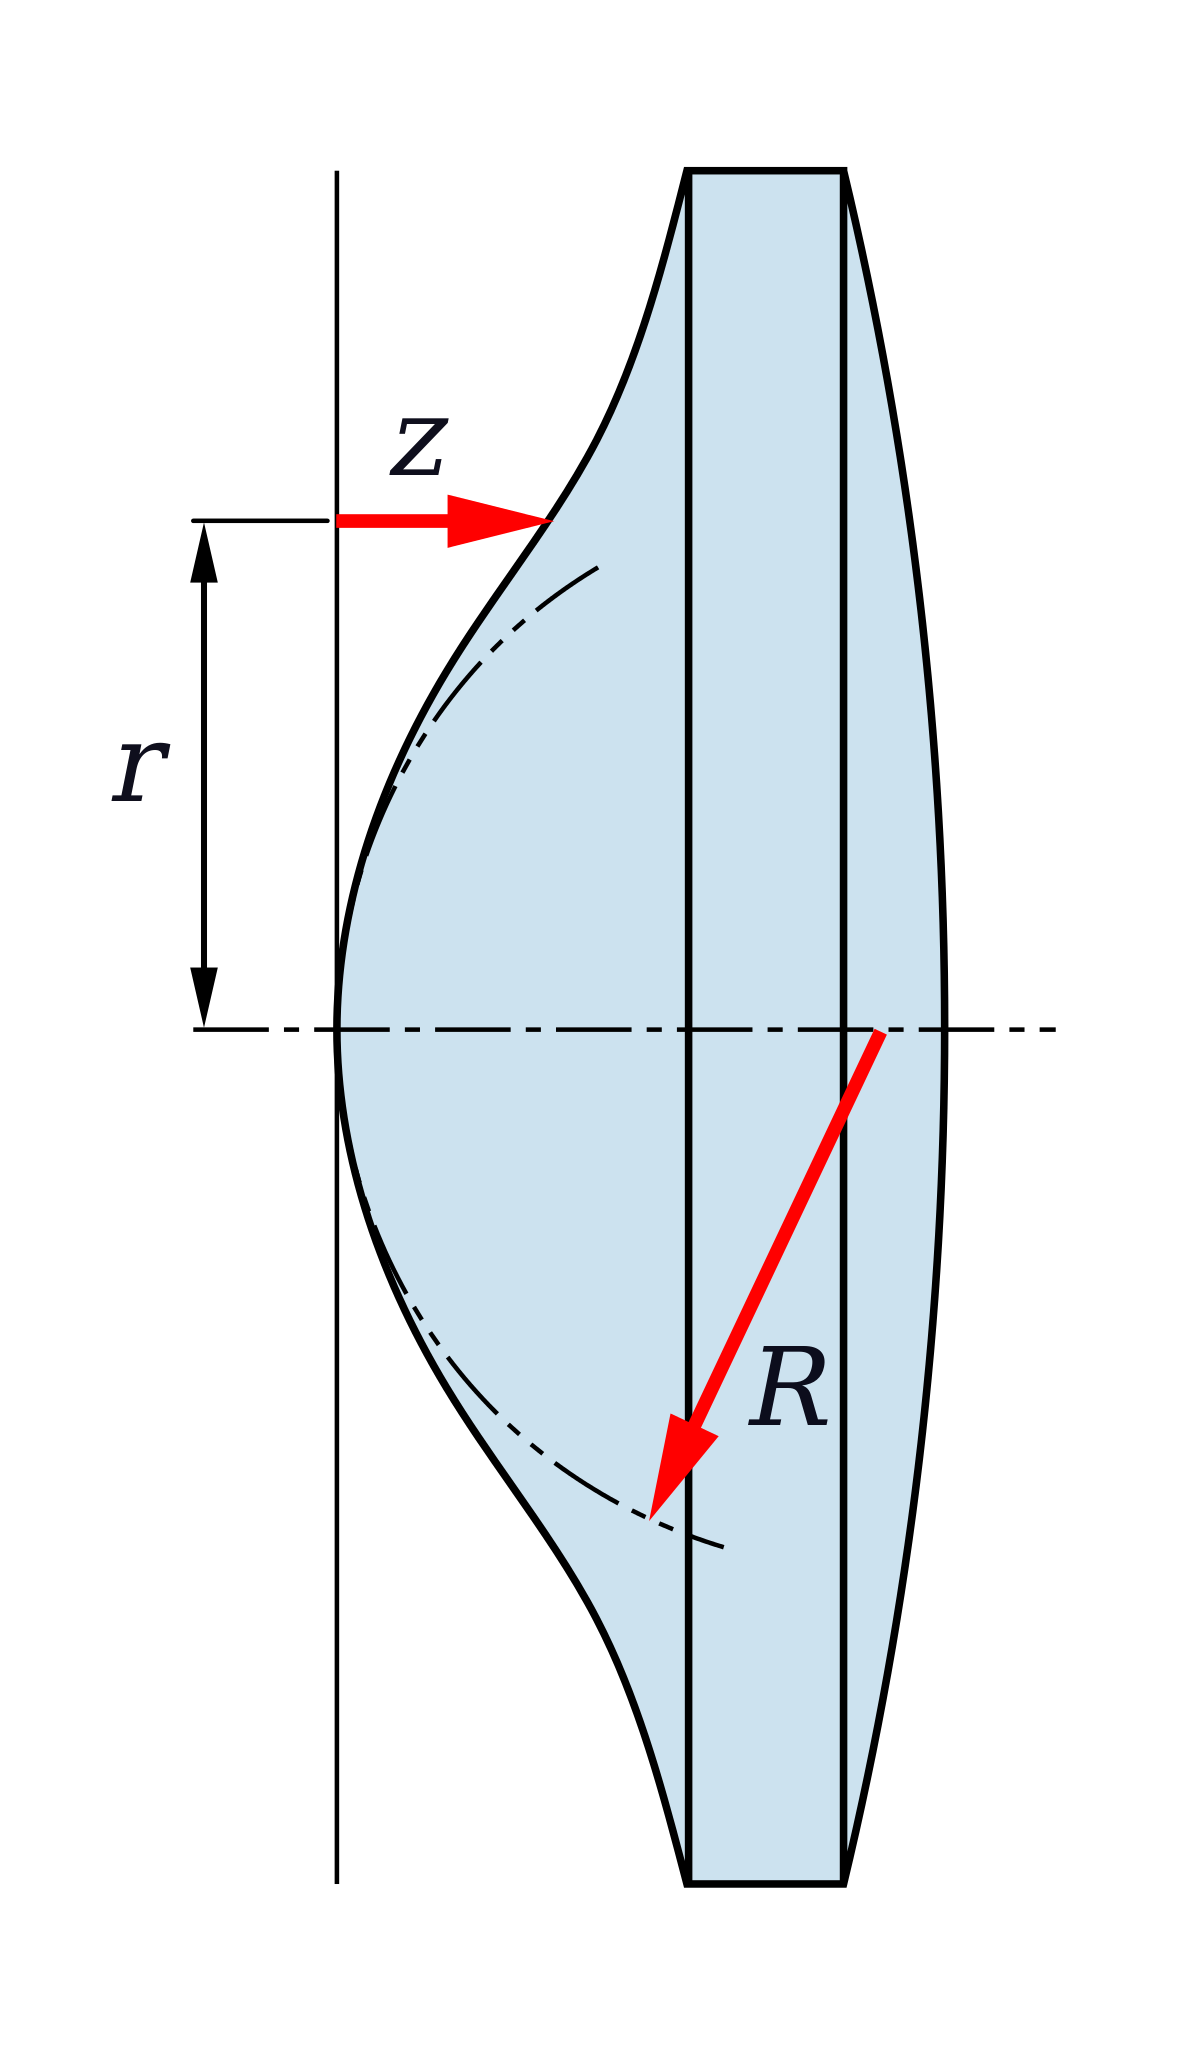
\includegraphics[width=3cm]{obrazky-figures/asphericLen.png}
\caption{Asférická šošvka, ktorej tvar potláča sférickú aberáciu. Prevzaté z }
\end{figure}

Týkala sa aj Hubblového teleskopu
\subsection{Coma}
Skreslenie off-axis objekov
\subsection{Petzvald field curvatore}
Riešenie: zakrivený senzor namiesto roviny.

\section{Chromatická aberácia}
Chromatická aberácia je jav šošovky, kedy jednotlivé vlnové dĺžky sú odlišne lomené pri dopade na
rozhranie šošovky. Dôsledkom toho je posunutie jednotlivých farebných zložiek v obraze, ktoré je
znázornené na obrázku \ref{chromaticAexample}.
Je spôsobená disperziou (rozptylom) svetla podľa vlnových dĺžok.

Obkec k obrazku = mozeme pozorovat, ze jednotlivé vlnové dlzky sú lomené pod iným uhlom, čo je
dosledok Snelloveho zakona.
\begin{figure}[h]
\centering
\label{chromaticAexample}
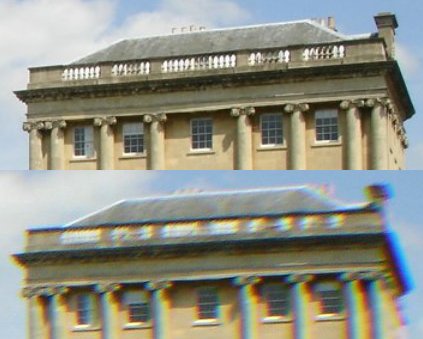
\includegraphics[width=6cm]{obrazky-figures/chromaticAberrationWikipedia.jpg}
\caption{lol}
\end{figure}

Riešenie: existujú SW \cite{automaticRemovalCA} ktoré sa pokúšajú o korekciu, 
existujú špeciálne šošovky, ktoré korektne lomia 2 vlnové dĺžky (doublet) alebo viacero
https://en.wikipedia.org/wiki/Achromatic\_lens
